\documentclass[11pt,a4paper]{article}

\usepackage[utf8]{inputenc}
\usepackage[T1]{fontenc}
\usepackage[spanish]{babel}
\usepackage{lmodern}
\usepackage[margin=2.5cm]{geometry}
\usepackage{tabularx,array,fancyhdr,booktabs}
\usepackage{xltabular}
\usepackage[table]{xcolor}
\usepackage{graphicx}
\usepackage[hidelinks]{hyperref}

\setlength{\headheight}{14pt}
\setlength{\parindent}{0pt}
\setlength{\parskip}{6pt}
\setlength{\emergencystretch}{1.5em}
\renewcommand{\arraystretch}{1.25}

\pagestyle{fancy}
\fancyhf{}
\fancyhead[L]{\small UTEQ \textperiodcentered{} Ingeniería de Requerimientos (ISR-401)}
\fancyhead[R]{\small GA-SUM-01 \textperiodcentered{} PE-U1}
\fancyfoot[L]{\small Grupo CEV \textperiodcentered{} Sistema DentiTech}
\fancyfoot[R]{\small Página \thepage}

\addto\captionsspanish{\renewcommand{\refname}{Referencias}}
\usepackage[backend=biber,style=ieee]{biblatex}
\addbibresource{referencias.bib}

\begin{document}

% ==================== PORTADA ====================
\begin{titlepage}
    \centering
    {\Large\textbf{UNIVERSIDAD TÉCNICA ESTATAL DE QUEVEDO}}\par
    \vspace{0.2cm}
    {\large Facultad de Ciencias de la Computación y Diseño Digital}\par
    {\large Carrera de Software (Rediseño)}\par
    
    \vspace{1.2cm}
    \rule{\textwidth}{1.5pt}\par
    \vspace{0.4cm}
    {\LARGE\bfseries Práctica Experimental Unidad I:\\Aplicación del Proceso de Ingeniería de Requisitos al Sistema DentiTech\par}
    \vspace{0.4cm}
    \rule{\textwidth}{1.5pt}\par
    
    \vspace{0.8cm}
    {\large\textbf{Código de Actividad:} GA-SUM-01 \textperiodcentered{} PE-U1}\par
    {\large\textbf{Asignatura:} Ingeniería de Requerimientos [ISR-401]}\par
    {\large\textbf{Nivel y Paralelo:} Cuarto Nivel --- Paralelo A}\par
    
    \vspace{1.2cm}
    \begin{tabularx}{\textwidth}{|l|l|X|}
        \hline
        \rowcolor{gray!15}
        \textbf{Rol en el Equipo} & \textbf{Integrante (Grupo CEV)} & \textbf{Correo Institucional} \\ \hline
        Analista Líder & Contreras Chavez Kevin German & \texttt{kcontrerasc3@uteq.edu.ec} \\ \hline
        Investigador A / Dev & Espinoza Pivaque Angelo Maximiliano & \texttt{anespinop01@gmail.com} \\ \hline
        Investigador B / Doc & Vaca Romero David Octavio & \texttt{dvacar@uteq.edu.ec} \\ \hline
    \end{tabularx}
    
    \vfill
    {\large\textbf{Docente Responsable:}\\Gleiston Cicerón Guerrero Ulloa, PhD}\par
    \vspace{0.6cm}
    {\large Quevedo --- Los Ríos --- Ecuador\\Período Académico 2026-2027 SPA}
\end{titlepage}

% ==================== ÍNDICE ====================
\tableofcontents
\newpage

% ==================== SECCIÓN 0 ====================
\section*{Sección 0: Definición y Contextualización del Proyecto (PFC)}
\addcontentsline{toc}{section}{Sección 0: Definición y Contextualización del Proyecto (PFC)}

\subsection*{0.1. Descripción del sistema (PFC)}
\addcontentsline{toc}{subsection}{0.1. Descripción del sistema (PFC)}

\textbf{DentiTech} es un sistema de información web y móvil diseñado para automatizar y optimizar la gestión integral de consultorios odontológicos en el contexto local de Quevedo. El problema principal que resuelve es la alta tasa de inasistencias de pacientes, el desorden en la agenda manual de turnos, la pérdida o deterioro de historiales clínicos físicos y la deficiente trazabilidad en el seguimiento evolutivo de los tratamientos dentales. Sus usuarios principales son los odontólogos (quienes diagnostican y registran evoluciones), los asistentes dentales (encargados de agendar, confirmar turnos y controlar pagos) y los pacientes (quienes solicitan y consultan sus citas). El contexto organizacional se centra en clínicas dentales medianas y consultorios particulares que requieren modernizar sus procesos operativos y clínicos bajo estándares de calidad y seguridad de la información.

\subsection*{0.2. Identificación de Stakeholders y Matriz Poder / Interés (PMBoK 7.ª ed.)}
\addcontentsline{toc}{subsection}{0.2. Identificación de Stakeholders y Matriz Poder / Interés}

Siguiendo los lineamientos del \textit{PMBoK Guide} 7.ª edición \cite{pmbok2021}, se identifican y clasifican las cinco partes interesadas (\textit{stakeholders}) fundamentales del proyecto \textbf{DentiTech}:

\begin{xltabular}{\textwidth}{|p{0.23\textwidth}|p{0.18\textwidth}|X|}
\hline
\rowcolor{gray!15}
\textbf{Stakeholder} & \textbf{Cuadrante} & \textbf{Rol en el Sistema y Estrategia de Gestión} \\ \hline
\endhead

\textbf{1. Odontólogo / Propietario} & Alto Poder \newline Alto Interés & \textbf{Rol:} Usuario clínico principal, experto del dominio y máxima autoridad financiera. \newline \textbf{Estrategia:} Gestionar de cerca; involucrarlo en la validación de reglas de negocio, flujos de atención y estructura del odontograma. \\ \hline

\textbf{2. Asistente Dental / Recepcionista} & Medio Poder \newline Alto Interés & \textbf{Rol:} Operador diario de la agenda, recepción de pacientes y control de recaudación. \newline \textbf{Estrategia:} Mantener informado y capacitar activamente, dado que interactúa continuamente con el módulo de citas. \\ \hline

\textbf{3. Paciente / Cliente} & Bajo Poder \newline Alto Interés & \textbf{Rol:} Usuario externo que demanda agendamiento ágil y recordatorios oportunos. \newline \textbf{Estrategia:} Monitorear su experiencia garantizando usabilidad intuitiva y notificaciones claras. \\ \hline

\textbf{4. Equipo de Desarrollo (Grupo CEV)} & Alto Poder \newline Medio Interés & \textbf{Rol:} Responsable del análisis, arquitectura, codificación, pruebas y despliegue técnico. \newline \textbf{Estrategia:} Mantener satisfechos los criterios técnicos y controlar rigurosamente el alcance en 8 semanas. \\ \hline

\textbf{5. Ente Regulador (MSP / LOPDP)} & Alto Poder \newline Bajo Interés & \textbf{Rol:} Establece normativas sanitarias y de confidencialidad de datos personales de salud. \newline \textbf{Estrategia:} Cumplir estrictamente las restricciones legales y de cifrado de historias clínicas. \\ \hline
\end{xltabular}

\subsection*{0.3. Tipo de sistema y justificación}
\addcontentsline{toc}{subsection}{0.3. Tipo de sistema y justificación}

De acuerdo con la taxonomía de sistemas descrita por Pohl \cite{pohl2025}, \textbf{DentiTech} se clasifica como un \textbf{Sistema de Información Interactivo de Gestión Transaccional} orientado a servicios web y bases de datos relacionales. 

\textbf{Justificación:} Se cataloga de este modo porque su núcleo operativo consiste en procesar transacciones concurrentes (reserva de bloques horarios, actualización de historias clínicas, registro de abonos), aplicar reglas de negocio estrictas propias del dominio sanitario y garantizar la integridad referencial y confidencialidad de datos médicos sensibles frente a accesos simultáneos de distintos roles.

\newpage

% ==================== SECCIÓN 2 ====================
\section{Fundamento Teórico}

\subsection{Ingeniería de Requisitos y Marco Normativo}

\begin{itemize}
    \item \textbf{Definición formal:} La Ingeniería de Requisitos (IR) constituye un enfoque sistemático, disciplinado y cuantificable para la elicitación, análisis, especificación, validación y gestión de los requisitos de un sistema o producto de software durante todo su ciclo de vida \cite{ieee29148, pohl2025, swebok2024}.
    \item \textbf{Explicación propia:} Esta disciplina establece el puente fundamental entre las necesidades reales de los interesados del negocio y el diseño técnico de la solución informática. Su propósito central radica en reducir la incertidumbre inicial mediante la transformación de expectativas ambiguas en especificaciones verificables y trazables. Aplicar estándares internacionales garantiza que los artefactos producidos posean rigor técnico, evitando retrabajos costosos y desviaciones en el alcance del proyecto durante las etapas de codificación.
    \item \textbf{Ejemplo vinculado al PFC (DentiTech):} En el desarrollo de \textbf{DentiTech}, la aplicación de la norma ISO/IEC/IEEE 29148:2018 \cite{ieee29148} permite formalizar la necesidad operativa de reducir las inasistencias de pacientes mediante una regla de negocio precisa: el envío automatizado de recordatorios 24 horas antes de la consulta y la liberación del turno tras 15 minutos de retraso injustificado.
\end{itemize}

\subsection{Proceso de Ingeniería de Requisitos (Actividades Centrales y Transversales)}

\begin{itemize}
    \item \textbf{Definición formal:} Según el marco metodológico de Pohl, el proceso de ingeniería de requisitos se estructura en tres actividades centrales (elicitación, documentación y negociación) respaldadas de manera continua por dos actividades transversales (validación y gestión de requisitos) \cite{pohl2025, ireb2023}.
    \item \textbf{Explicación propia:} La elicitación busca descubrir el conocimiento del dominio mediante técnicas de indagación con los actores involucrados, mientras que la documentación plasma dichos hallazgos en formatos estructurados o modelos conceptuales. Por su parte, la negociación resuelve conflictos de intereses o prioridades entre los distintos interesados antes de comprometer recursos técnicos. Finalmente, la validación asegura que los requisitos reflejen fielmente lo que el cliente necesita, y la gestión controla su trazabilidad y evolución frente a los cambios del entorno.
    \item \textbf{Ejemplo vinculado al PFC (DentiTech):} Durante la fase de elicitación en consultorios odontológicos locales, se entrevistó a odontólogos y asistentes dentales para mapear el flujo real de atención. Posteriormente, se negoció entre el propietario (quien priorizaba el control financiero de tratamientos) y la recepcionista (quien requería rapidez al reagendar turnos), validando ambos flujos mediante prototipos de interfaz antes de aprobar la línea base.
\end{itemize}

\subsection{Clasificación y Taxonomía de Requisitos}

\begin{itemize}
    \item \textbf{Definición formal:} Los requisitos se clasifican jerárquicamente en requisitos de negocio, requisitos de los interesados (\textit{stakeholders}), requisitos del sistema ---subdivididos en Requisitos Funcionales (RF) y Requisitos No Funcionales (RNF) o atributos de calidad--- y restricciones de diseño o implementación \cite{ieee29148, iso25010, swebok2024}.
    \item \textbf{Explicación propia:} Distinguir adecuadamente cada categoría evita mezclar objetivos estratégicos de alto nivel con reglas técnicas de programación o limitaciones del entorno operativo. Mientras los requisitos funcionales detallan los comportamientos, transformaciones y servicios específicos que el software debe ejecutar, los no funcionales establecen criterios medibles de rendimiento, seguridad, usabilidad y disponibilidad bajo el modelo de calidad ISO/IEC 25010:2023 \cite{iso25010}. Las restricciones, en cambio, acotan las opciones de solución por motivos legales, tecnológicos o presupuestarios.
    \item \textbf{Ejemplo vinculado al PFC (DentiTech):} Un requisito funcional en \textbf{DentiTech} consiste en registrar el odontograma digital por pieza dental tratada; un requisito no funcional exige que la consulta del historial clínico cargue en menos de 1,5 segundos; y una restricción normativa obliga a cifrar los datos clínicos sensibles conforme a la legislación ecuatoriana de protección de datos.
\end{itemize}

\subsection{Propiedades de Calidad de los Requisitos}

\begin{itemize}
    \item \textbf{Definición formal:} Conforme a la norma IEEE/ISO/IEC 29148:2018, todo requisito individual bien formulado debe satisfacer atributos esenciales de calidad, entre los que destacan: necesidad, ausencia de ambigüedad, completitud, singularidad, viabilidad, verificabilidad, consistencia y trazabilidad \cite{ieee29148, ireb2023}.
    \item \textbf{Explicación propia:} Un requisito carente de estas propiedades introduce riesgos críticos de interpretación errónea por parte del equipo de desarrollo y dificulta la construcción de casos de prueba objetivos. La ausencia de ambigüedad y la verificabilidad son indispensables para comprobar mediante inspección o medición si el producto terminado cumple exactamente lo pactado. Asimismo, la trazabilidad bidireccional permite rastrear el origen de cada funcionalidad desde la necesidad del negocio hasta su implementación y prueba final.
    \item \textbf{Ejemplo vinculado al PFC (DentiTech):} En lugar de redactar una expresión ambigua como \textit{``el sistema debe ser rápido al agendar citas''}, en \textbf{DentiTech} se formula bajo criterios verificables: \textit{``El sistema debe confirmar y registrar una nueva cita odontológica en la base de datos en un tiempo máximo de 2 segundos bajo una carga concurrente de 20 usuarios''}.
\end{itemize}

\subsection{Tipología de Sistemas y Contexto del Sistema}

\begin{itemize}
    \item \textbf{Definición formal:} El contexto del sistema abarca la parte del entorno operativo que influye directamente en la definición y comprensión de los requisitos, delimitando la frontera entre el sistema a construir, los actores humanos, los sistemas externos y las normativas vigentes \cite{ieee15288, ieee12207, pohl2025}.
    \item \textbf{Explicación propia:} Comprender a qué tipología pertenece un proyecto (sistemas embebidos, sistemas de información transaccionales, aplicaciones web intensivas en datos, entre otros) determina qué técnicas de elicitación y qué atributos de calidad resultan críticos. Establecer con precisión el límite del sistema (\textit{system boundary}) evita asumir responsabilidades que pertenecen a plataformas externas o procesos manuales de la organización. De esta manera, se definen con claridad las interfaces de entrada y salida de datos antes de diseñar la arquitectura.
    \item \textbf{Ejemplo vinculado al PFC (DentiTech):} \textbf{DentiTech} se enmarca como un sistema de información interactivo orientado a la gestión clínica transaccional; su frontera excluye el procesamiento financiero directo de tarjetas bancarias, delegando dicha función a una pasarela externa y limitándose a consumir el comprobante de aprobación mediante una interfaz API REST.
\end{itemize}

\subsection{Artefactos y Herramientas de Especificación (Sintaxis EARS y Modelos)}

\begin{itemize}
    \item \textbf{Definición formal:} Los artefactos de especificación comprenden documentos estructurados (ERS), glosarios, listas priorizadas (MoSCoW) y plantillas lingüísticas controladas como EARS (\textit{Easy Approach to Requirements Syntax}), diseñadas para eliminar ambigüedades gramaticales mediante patrones predefinidos \cite{pohl2025, pmbok2021, mavin2009}.
    \item \textbf{Explicación propia:} La combinación de lenguaje natural estructurado con representaciones visuales (diagramas de contexto, casos de uso y mapas conceptuales) facilita la comunicación efectiva tanto con usuarios no técnicos como con arquitectos de software. El empleo de patrones sintácticos estandarizados uniformiza la redacción entre múltiples analistas y simplifica las revisiones de calidad. Paralelamente, técnicas de priorización como MoSCoW permiten gestionar el alcance del proyecto de forma iterativa según el valor aportado al negocio.
    \item \textbf{Ejemplo vinculado al PFC (DentiTech):} Para especificar los comportamientos reactivos de la agenda odontológica en \textbf{DentiTech}, se aplica el patrón dirigido por eventos de EARS: \textit{``Cuando un paciente solicite la cancelación de su turno con más de 12 horas de antelación, el sistema deberá liberar el bloque horario y notificar automáticamente al asistente dental''}.
\end{itemize}

\newpage

% ==================== SECCIÓN 3 ====================
\section{Artefactos y Aplicación del Proceso de Requisitos}

\subsection{Tabla de Identificación y Clasificación de Requisitos}

La Tabla~\ref{tab:requisitos} presenta 15 requisitos únicos formulados para \textbf{DentiTech}, aplicando la sintaxis controlada EARS \cite{mavin2009} para requisitos funcionales, atributos cuantificados de ISO/IEC 25010:2023 \cite{iso25010} para requisitos no funcionales, priorización MoSCoW y trazabilidad hacia su origen.

\begingroup
\small
\setlength{\tabcolsep}{4pt}
\begin{xltabular}{\textwidth}{|p{0.10\textwidth}|p{0.15\textwidth}|X|p{0.11\textwidth}|p{0.18\textwidth}|}
\caption{Especificación y clasificación de requisitos del sistema DentiTech.} \label{tab:requisitos} \\
\hline
\rowcolor{gray!15}
\textbf{ID} & \textbf{Tipo} & \textbf{Descripción Formal (Sintaxis EARS / Estándar)} & \textbf{MoSCoW} & \textbf{Fuente} \\ \hline
\endfirsthead
\hline
\rowcolor{gray!15}
\textbf{ID} & \textbf{Tipo} & \textbf{Descripción Formal (Sintaxis EARS / Estándar)} & \textbf{MoSCoW} & \textbf{Fuente} \\ \hline
\endhead

\textbf{RF-01} & Funcional & Cuando el paciente seleccione un horario disponible, el sistema deberá registrar la cita odontológica en estado pendiente. & Must & Entrevista a Asistente Dental \\ \hline

\textbf{RF-02} & Funcional & El sistema deberá enviar un recordatorio automatizado por correo electrónico 24 horas antes de la consulta programada. & Should & Objetivo de Negocio \\ \hline

\textbf{RF-03} & Funcional & Mientras el odontólogo mantenga abierta la sesión clínica, el sistema permitirá actualizar el odontograma digital por pieza dental tratada. & Must & Entrevista a Odontólogo \\ \hline

\textbf{RF-04} & Funcional & Si el paciente cancela su turno con más de 12 horas de anticipación, el sistema liberará automáticamente el bloque horario en la agenda. & Should & Regla de Gestión Clínica \\ \hline

\textbf{RF-05} & Funcional & El sistema deberá generar un reporte mensual consolidado en formato PDF de atenciones realizadas y abonos recaudados. & Could & Propietario del Consultorio \\ \hline

\textbf{RNF-01} & Rendimiento \newline (ISO 25010) & El tiempo de respuesta al consultar el historial clínico de un paciente no deberá superar los 1,5 segundos bajo una carga de 20 usuarios concurrentes \cite{iso25010}. & Must & Análisis Técnico \\ \hline

\textbf{RNF-02} & Seguridad \newline (ISO 25010) & El sistema deberá cifrar las contraseñas mediante \textit{bcrypt} y los diagnósticos clínicos sensibles mediante AES-256 en la base de datos \cite{iso25010}. & Must & Normativa LOPDP \\ \hline

\textbf{RNF-03} & Fiabilidad \newline (ISO 25010) & El sistema garantizará una disponibilidad operativa mínima del 99,0\% durante la jornada laboral de atención (08:00 a 19:00) \cite{iso25010}. & Should & Acuerdo de Servicio \\ \hline

\textbf{RNF-04} & Usabilidad \newline (ISO 25010) & La interfaz web deberá adaptarse de forma responsiva a pantallas móviles desde 360 px de ancho, permitiendo agendar en máximo 4 pasos \cite{iso25010}. & Should & Evaluación de Usuarios \\ \hline

\textbf{RNF-05} & Mantenibilidad \newline (ISO 25010) & El código fuente del \textit{backend} deberá estructurarse bajo arquitectura modular en capas con cobertura de pruebas unitarias superior al 70\% \cite{iso25010}. & Could & Equipo de Desarrollo \\ \hline

\textbf{INT-01} & Interfaz \newline (Usuario) & El sistema presentará una interfaz de autenticación con control de acceso basado en roles diferenciados (Paciente, Asistente, Odontólogo). & Must & Especificación UI/UX \\ \hline

\textbf{INT-02} & Interfaz \newline (Software) & El sistema consumirá una pasarela de pagos externa mediante protocolo API REST/JSON sobre HTTPS para validar transferencias. & Could & Requisito de Integración \\ \hline

\textbf{RES-01} & Restricción & El tratamiento y almacenamiento de historiales clínicos deberá cumplir obligatoriamente con la Ley Orgánica de Protección de Datos Personales del Ecuador. & Must & Restricción Legal \\ \hline

\textbf{RES-02} & Restricción & El desarrollo completo deberá emplear tecnologías web de código abierto dentro de un cronograma de 8 semanas sin costos de licenciamiento. & Must & Restricción del PFC \\ \hline

\textbf{CON-01} & Conformidad & Los artefactos de especificación y código se adherirán a los estándares de calidad IEEE/ISO/IEC 29148:2018 exigidos en la asignatura \cite{ieee29148}. & Must & Guía Práctica UTEQ \\ \hline
\end{xltabular}
\endgroup

\subsection{Evaluación de Propiedades de Calidad (ISO/IEC/IEEE 29148:2018)}

La Tabla~\ref{tab:propiedades} verifica cada requisito de \textbf{DentiTech} frente a los atributos individuales de calidad establecidos por la norma IEEE/ISO/IEC 29148:2018 \cite{ieee29148}.

\begingroup
\small
\setlength{\tabcolsep}{4pt}
\begin{xltabular}{\textwidth}{|p{0.10\textwidth}|c|c|c|c|X|}
\caption{Evaluación de propiedades de calidad IEEE 29148:2018 por requisito.} \label{tab:propiedades} \\
\hline
\rowcolor{gray!15}
\textbf{ID} & \textbf{Nec.} & \textbf{S/Amb.} & \textbf{Verif.} & \textbf{Traz.} & \textbf{Argumentación Verificable de Cumplimiento} \\ \hline
\endfirsthead
\hline
\rowcolor{gray!15}
\textbf{ID} & \textbf{Nec.} & \textbf{S/Amb.} & \textbf{Verif.} & \textbf{Traz.} & \textbf{Argumentación Verificable de Cumplimiento} \\ \hline
\endhead

\textbf{RF-01} & \checkmark & \checkmark & \checkmark & \checkmark & Resuelve el desorden de turnos; posee disparador claro (\textit{selección de horario}) y estado observable (\textit{pendiente}). \\ \hline
\textbf{RF-02} & \checkmark & \checkmark & \checkmark & \checkmark & Define un umbral exacto (24 horas) y canal verificable (correo), auditable mediante registros de envío SMTP. \\ \hline
\textbf{RF-03} & \checkmark & \checkmark & \checkmark & \checkmark & Acota el estado de sesión clínica activa y la unidad de registro (pieza dental), evitando ambigüedades médicas. \\ \hline
\textbf{RF-04} & \checkmark & \checkmark & \checkmark & \checkmark & Establece condición temporal precisa (>12 h) y efecto automático verificable mediante pruebas funcionales. \\ \hline
\textbf{RF-05} & \checkmark & \checkmark & \checkmark & \checkmark & Especifica periodicidad mensual, formato de salida (PDF) y métricas financieras trazables al propietario. \\ \hline
\textbf{RNF-01} & \checkmark & \checkmark & \checkmark & \checkmark & Cuantifica latencia máxima (1,5 s) y concurrencia (20 usuarios), verificable mediante pruebas de carga con JMeter. \\ \hline
\textbf{RNF-02} & \checkmark & \checkmark & \checkmark & \checkmark & Especifica algoritmos estándar (\textit{bcrypt}, AES-256), verificable mediante inspección del esquema de base de datos. \\ \hline
\textbf{RNF-03} & \checkmark & \checkmark & \checkmark & \checkmark & Define métrica porcentual (99,0\%) y franja horaria exacta, auditable mediante monitoreo continuo (\textit{uptime}). \\ \hline
\textbf{RNF-04} & \checkmark & \checkmark & \checkmark & \checkmark & Establece resolución mínima (360 px) y límite de interacción (4 pasos), comprobable en pruebas de usabilidad. \\ \hline
\textbf{RNF-05} & \checkmark & \checkmark & \checkmark & \checkmark & Cuantifica cobertura de pruebas (>70\%) y patrón arquitectónico, verificable mediante análisis estático de código. \\ \hline
\textbf{INT-01} & \checkmark & \checkmark & \checkmark & \checkmark & Enumera explícitamente los 3 roles del sistema, verificable comprobando permisos de acceso por perfil. \\ \hline
\textbf{INT-02} & \checkmark & \checkmark & \checkmark & \checkmark & Define protocolo (API REST/JSON) y seguridad (HTTPS), comprobable en pruebas de integración con entorno \textit{sandbox}. \\ \hline
\textbf{RES-01} & \checkmark & \checkmark & \checkmark & \checkmark & Derivada de normativa legal obligatoria; verificable auditando consentimiento informado y cifrado en tránsito. \\ \hline
\textbf{RES-02} & \checkmark & \checkmark & \checkmark & \checkmark & Acota licenciamiento (código abierto) y plazo (8 semanas), verificable en el repositorio Git del proyecto. \\ \hline
\textbf{CON-01} & \checkmark & \checkmark & \checkmark & \checkmark & Trazable a la rúbrica institucional; verificable mediante lista de cotejo documental de la asignatura ISR-401. \\ \hline
\end{xltabular}
\endgroup

\subsection{Límite del Sistema y Declaración de Visión (Formato Moore)}

\textbf{Límite del sistema (Entidades externas e interfaces):}
\begin{enumerate}
    \item \textbf{Paciente:} Envía solicitudes de reserva/cancelación de turnos y recibe confirmaciones (Protocolo HTTPS / Interfaz Web Responsiva, frecuencia asíncrona por demanda).
    \item \textbf{Asistente Dental:} Gestiona la agenda diaria, confirma asistencias y registra pagos (Protocolo HTTPS / Interfaz Web, frecuencia continua en jornada laboral).
    \item \textbf{Odontólogo:} Consulta historiales clínicos y actualiza diagnósticos/odontogramas (Protocolo HTTPS / Interfaz Web, frecuencia por consulta atendida).
    \item \textbf{Pasarela de Pagos Externa:} Recibe solicitudes de cobro y retorna comprobantes de validación (Protocolo API REST / JSON sobre TLS 1.3, frecuencia por evento de pago).
    \item \textbf{Servidor de Correo Electrónico (SMTP):} Recibe peticiones de notificación desde el \textit{backend} y despacha recordatorios (Protocolo SMTP/TLS, frecuencia programada cada hora).
\end{enumerate}

\textbf{Declaración de Visión (Formato Geoffrey Moore \cite{moore2014}):}
\begin{quote}
\textit{``Para \textbf{pacientes y profesionales de consultorios odontológicos locales} que \textbf{enfrentan desorden en el agendamiento de turnos, altas tasas de inasistencia y pérdida de historiales clínicos físicos}, \textbf{DentiTech} es un \textbf{sistema web y móvil de gestión clínica transaccional} que \textbf{automatiza la reserva de citas, centraliza el odontograma digital y optimiza el control administrativo}. A diferencia de \textbf{las agendas manuscritas tradicionales o la coordinación informal mediante mensajería instantánea}, nuestro producto \textbf{garantiza trazabilidad clínica en tiempo real, cumplimiento de protección de datos personales y reducción efectiva de inasistencias mediante recordatorios automatizados}.''}
\end{quote}

\subsection{Aplicación de las Ocho Perspectivas de Contexto (Klaus Pohl)}

Siguiendo el marco de contexto de Pohl \cite{pohl2025}, se analizan las ocho perspectivas aplicadas a \textbf{DentiTech}:

\begin{enumerate}
    \item \textbf{Perspectiva Operativa:} \textit{Preguntas clave:} ¿Cómo interactúa el asistente en horas pico? ¿Cuántos pasos requiere agendar un turno? ¿Cómo visualiza el odontólogo el odontograma? \textit{Requisitos emergentes:} Agenda visual con filtros por especialista y atajos rápidos de confirmación en un solo clic.
    \item \textbf{Perspectiva Temporal:} \textit{Preguntas clave:} ¿Con cuánta antelación se envían los recordatorios? ¿Cuándo expira una cita no confirmada? ¿Cuál es la duración estándar por tratamiento? \textit{Requisitos emergentes:} Tareas programadas (\textit{cron jobs}) cada hora para notificaciones y bloqueo automático de intervalos según tipo de procedimiento.
    \item \textbf{Perspectiva Organizacional:} \textit{Preguntas clave:} ¿Qué permisos diferencian al propietario del asistente? ¿Quién autoriza descuentos o anulaciones de cobro? ¿Cómo se auditan los cambios clínicos? \textit{Requisitos emergentes:} Control de acceso basado en roles (RBAC) y prohibición de borrado físico de evoluciones médicas.
    \item \textbf{Perspectiva Tecnológica:} \textit{Preguntas clave:} ¿Qué navegadores utilizan los consultorios? ¿Cómo responde la aplicación ante caídas breves de red? ¿Qué dispositivos usan los pacientes? \textit{Requisitos emergentes:} Diseño responsivo compatible con dispositivos móviles de gama baja y manejo controlado de reconexión de sesiones.
    \item \textbf{Perspectiva de Datos:} \textit{Preguntas clave:} ¿Cómo se relaciona cada pieza dental con su historial de intervenciones? ¿Qué datos personales son obligatorios al registrar un paciente? \textit{Requisitos emergentes:} Modelo relacional normalizado en tercera forma normal (3FN) con integridad referencial estricta.
    \item \textbf{Perspectiva de Infraestructura:} \textit{Preguntas clave:} ¿Dónde se alojará la base de datos? ¿Cómo se realizarán las copias de seguridad? ¿Qué ancho de banda requiere el consultorio? \textit{Requisitos emergentes:} Despliegue en servidor en la nube con certificados SSL/TLS y respaldos automatizados diarios.
    \item \textbf{Perspectiva Legal y Normativa:} \textit{Preguntas clave:} ¿Cómo se cumple la Ley Orgánica de Protección de Datos Personales? ¿Cómo se valida el consentimiento del paciente? \textit{Requisitos emergentes:} Registro digital de aceptación de políticas de privacidad y cifrado de información médica sensible.
    \item \textbf{Perspectiva de Calidad y Seguridad:} \textit{Preguntas clave:} ¿Cómo se previenen accesos no autorizados? ¿Qué ocurre ante intentos reiterados de inicio de sesión fallidos? \textit{Requisitos emergentes:} Bloqueo temporal de cuenta tras 5 intentos fallidos y bitácora (\textit{log}) de auditoría de transacciones críticas.
\end{enumerate}

\subsection{Mapeo del Proceso de Requisitos con Actores y Artefactos}

La Tabla~\ref{tab:proceso} evidencia la ejecución secuencial y transversal del proceso de ingeniería de requisitos \cite{pohl2025} en el proyecto \textbf{DentiTech}.

\begingroup
\small
\setlength{\tabcolsep}{4pt}
\begin{xltabular}{\textwidth}{|p{0.17\textwidth}|p{0.13\textwidth}|p{0.22\textwidth}|X|}
\caption{Aplicación del proceso de requisitos de Pohl al sistema DentiTech.} \label{tab:proceso} \\
\hline
\rowcolor{gray!15}
\textbf{Actividad} & \textbf{Dimensión} & \textbf{Actores Involucrados} & \textbf{Evidencia de Aplicación y Artefacto Parcial} \\ \hline
\endfirsthead
\hline
\rowcolor{gray!15}
\textbf{Actividad} & \textbf{Dimensión} & \textbf{Actores Involucrados} & \textbf{Evidencia de Aplicación y Artefacto Parcial} \\ \hline
\endhead

\textbf{1. Elicitación} & Central & Analista Líder, Odontólogo, Asistente, Pacientes & Entrevistas semiestructuradas y observación directa de cuadernos de citas en consultorios locales. \textit{Artefacto:} Guion de entrevista y lista inicial de necesidades. \\ \hline

\textbf{2. Documentación} & Central & Investigadores A, B y Documentador & Redacción estructurada bajo patrones EARS, métricas ISO 25010 y delimitación de fronteras. \textit{Artefacto:} Especificación de requisitos (Tabla~\ref{tab:requisitos}). \\ \hline

\textbf{3. Negociación} & Central & Analista Líder, Propietario, Equipo Técnico & Priorización de funcionalidades esenciales (agenda y odontograma) frente a integraciones secundarias para cumplir el plazo de 8 semanas. \textit{Artefacto:} Matriz MoSCoW aprobada. \\ \hline

\textbf{4. Validación} & Transversal & Todos los Stakeholders y Equipo CEV & Revisión de calidad bajo criterios IEEE 29148 y validación de flujos mediante prototipos de interfaz de baja fidelidad. \textit{Artefacto:} Matriz de calidad (Tabla~\ref{tab:propiedades}). \\ \hline

\textbf{5. Gestión} & Transversal & Analista Líder y Documentador & Asignación de identificadores únicos (\texttt{RF-01} a \texttt{CON-01}), control de versiones en GitHub y trazabilidad bidireccional hacia las fuentes. \textit{Artefacto:} Repositorio versionado. \\ \hline
\end{xltabular}
\endgroup

\subsection{Mapa Conceptual Integrador}

La Figura~\ref{fig:mapa} sintetiza la articulación entre los fundamentos normativos, el proceso de Pohl, la taxonomía de requisitos y los atributos de calidad aplicados a \textbf{DentiTech}.

\begin{figure}[htbp]
    \centering
    
\includegraphics[width=0.95\textwidth]{figura1.png}
    \caption{Mapa conceptual integrador de los fundamentos y proceso de Ingeniería de Requisitos aplicado a DentiTech.}
    \label{fig:mapa}
\end{figure}

\newpage
% ==================== CONCLUSIONES ====================
\section{Conclusiones}

\begin{enumerate}
    \item \textbf{Contreras Chavez Kevin German (Analista Líder):} La aplicación rigurosa de estándares internacionales transforma necesidades operativas ambiguas en especificaciones técnicas verificables y libres de interpretaciones subjetivas. Al contrastar las entrevistas realizadas en consultorios odontológicos locales con los atributos de calidad de la norma IEEE/ISO/IEC 29148:2018 \cite{ieee29148}, se logró estructurar quince requisitos trazables bajo sintaxis EARS \cite{mavin2009} y métricas ISO/IEC 25010 \cite{iso25010}, eliminando ambigüedades críticas en el agendamiento de turnos. Para el desarrollo de \textbf{DentiTech} y nuestra formación profesional, este rigor metodológico garantiza una línea base sólida que minimiza el retrabajo en etapas posteriores de codificación y pruebas.

    \item \textbf{Espinoza Pivaque Angelo Maximiliano (Investigador / Desarrollador):} La delimitación temprana de las fronteras del sistema y sus interfaces externas constituye un factor determinante para controlar el alcance real de un proyecto de software. Mediante el análisis de entidades externas y la aplicación de las ocho perspectivas de contexto propuestas por Pohl \cite{pohl2025}, se identificaron requerimientos ocultos en \textbf{DentiTech}, tales como el manejo de sesiones inactivas, la sincronización ante fallos de red y la integración vía API REST con pasarelas de pago. Esta visión sistémica resulta indispensable en la ingeniería de software moderna para diseñar arquitecturas modulares y evitar asumir responsabilidades operativas que corresponden a servicios de terceros.

    \item \textbf{Vaca Romero David Octavio (Investigador / Documentador):} La priorización estructurada y la evaluación temprana de propiedades de calidad permiten alinear las expectativas de los distintos interesados con las restricciones reales de tiempo y presupuesto. Durante la etapa de negociación de \textbf{DentiTech}, el empleo de la matriz poder/interés del PMBoK \cite{pmbok2021} junto con el esquema MoSCoW facilitó equilibrar las demandas administrativas del odontólogo propietario frente a las necesidades operativas del asistente dental dentro de un plazo acotado de ocho semanas. En el ejercicio profesional, dominar estas técnicas de gestión asegura entregas de alto valor funcional sin comprometer la viabilidad técnica del equipo.
\end{enumerate}

% ==================== REFERENCIAS ====================
\newpage
\printbibliography[title={Referencias Bibliográficas (Formato IEEE)}]

% ==================== ANEXOS ====================
\newpage
\appendix
\section{Listado de Fuentes Bibliográficas Exportadas}
Las referencias utilizadas en el presente informe fueron gestionadas y validadas siguiendo el estilo IEEE comprimido exigido por la cátedra, correspondiendo a las diez fuentes primarias indexadas en la sección de Referencias Bibliográficas (\texttt{[1]} a \texttt{[10]}).

\section{Evidencia de Gestión Bibliográfica (Mendeley / Zotero)}
\begin{figure}[htbp]
    \centering
    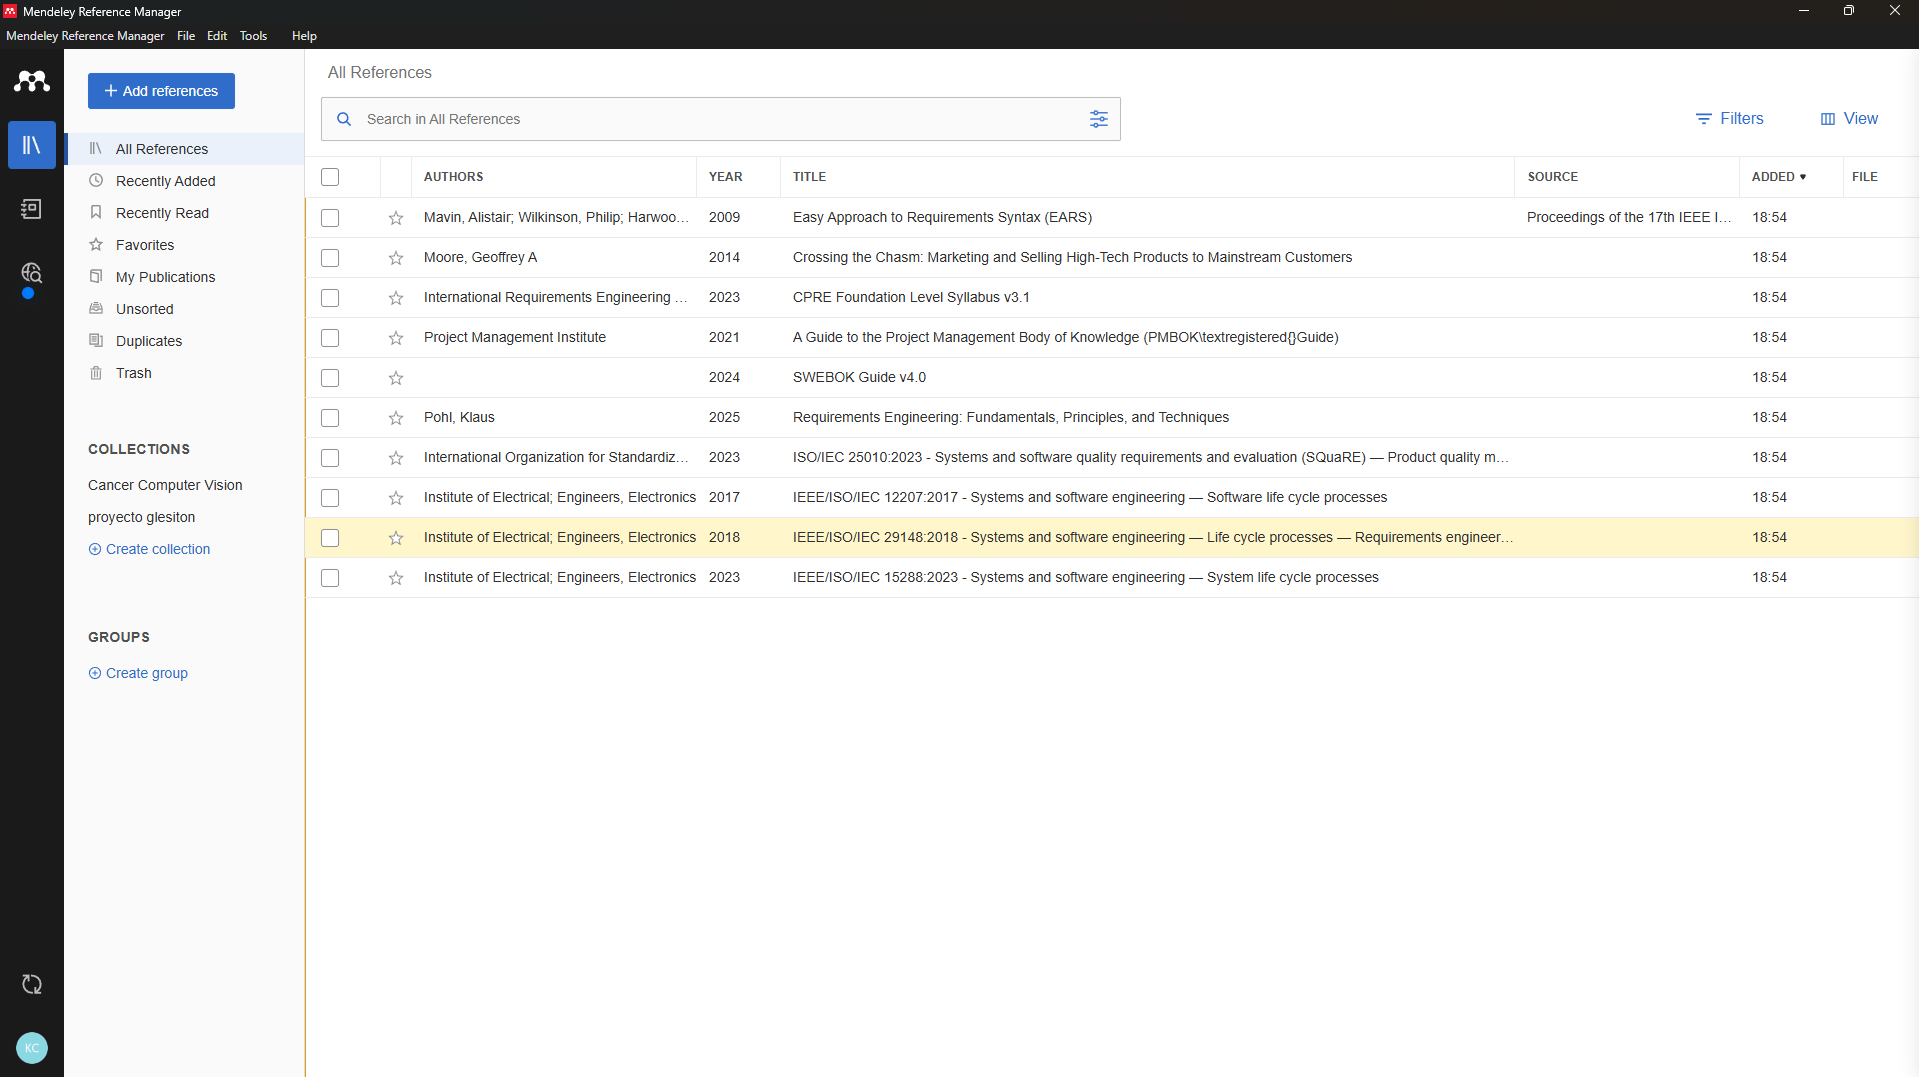
\includegraphics[width=0.92\textwidth]{anexo_b.png}
    \caption{Captura de la biblioteca de referencias gestionada en Mendeley/Zotero para el proyecto DentiTech.}
    \label{fig:anexo_b}
\end{figure}

\end{document}